%% SECTION HEADER /////////////////////////////////////////////////////////////////////////////////////
\section{Results}
\label{sec:resuls}

%% SECTION CONTENT ////////////////////////////////////////////////////////////////////////////////////
\subsection{Validation with the \ac{sldv}}
The fullfield of the wave propagation in the reference sample is presented in Fig.~\ref{fig:wavefield}.
The experimental measurements and the present model snapshots show that the wavefront distortion is rising with the frequency.
Because the wavelength decreases as the frequency increases, a higher frequency signal is more likely to reflect off the core walls.
This effect is not observed in the case of the homogenized model.
\vspace{-6pt}
\begin{figure}[H]
	\begin{center}
		\includegraphics{Chapter_6/fullfield}
	\end{center}
	\caption{The top surface out of plane particle velocity snapshots in time 100 \(\mu\)s for (\textbf{a}) the experimental results obtained by using \ac{sldv}, (\textbf{b}) the present model and (\textbf{c}) the homogenized model in the pristine~sample.}
	\label{fig:wavefield}
\end{figure}

\begin{figure}[H]
	\begin{center}
		\includegraphics{Chapter_6/fullfield_dam}
	\end{center}
	\caption{The top surface out of plane particle velocity snapshots in time 100~\(\mu\)s for (\textbf{a}) the experimental results obtained by using \ac{sldv} in the sample with 90 mm width damage, (\textbf{b}) the present model and (\textbf{c}) the homogenized model with removed core elements in damaged area for both numerical models.}
	\label{fig:wavefield_dam5}
\end{figure}

In case of the damage sample, the wavefront is not distorted in the damage area bounded by two dotted line in Fig.~\ref{fig:wavefield_dam5} for all three cases.
Due to the lack of wave leakage into the core, thus the wave propagates smoothly through the skin.
For the experimental sample and the present model, interference of waves reflected from the cells and the damage boundary is observed.
The wave interference observed in the homogenized model refers to waves reflected only from the defect.

\subsection{Validation with the \acp{pzt}}
The group velocities of the first packet arriving at the sensor were determined to validate the numerical models.  
The group velocity is calculated as follows:
\begin{eqnarray}
	C_g = \frac{\mathrm{ToF}}{l},
\end{eqnarray}
where \(l=200\) mm is a distance between the transducers, and ToF is the wave package time of flight extracted from Fig. \ref{fig:ToF_exp}, \ref{fig:ToF_num}, \ref{fig:ToF_hom}, for experimental measurements, the present model and the homogonised model, respectively.

The determined velocities and the errors of the numerical models relative to the experimental results are given in Table \ref{tab:group_velocity}, where the error is defined as:
\begin{eqnarray}
	error = \left|\frac{C_g^{num}-C_g^{exp}}{C_g^{exp}}\right|\times100\%,
\end{eqnarray}
where \(C_g^{num}\) is group velocity obtained from numerical simulations, and \(C_g^{exp}\) is group velocity obtained from experimental measurements.
The group velocity for the present model agrees well with experimental measurements, with an error of less than 10\%.
For the homogenized model, only the 150 kHz signal has an error 10.79\% higher than the experiment.
It can be also seen that the velocity for the present model monotonically decreases with increasing frequency, as in the experiment, which is expected from the S0 dispersion curve.
The results for the homogenized model do not show such a trend.

Velocity errors of models relative to experimental results can result from several factors. The most important ones include differences in material properties of used components. In the models, an average thickness of the adhesive layer was assumed; obtaining such a layer in the specimen preparation is difficult under workshop conditions. The models also assume a uniform cell geometry for the core area, but in reality, the core is easily deformed in the plane, so the cell geometry varies. The propagation angle varies the velocity in the \ac{cfrp} skin; in the models, it was assumed to be 0. The speed is also affected by the accuracy of the \acp{pzt} placement. 
\begin{figure}[H]
	\begin{center}
		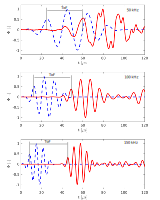
\includegraphics{Chapter_6/ToF_exp}
	\end{center}
	\caption{Sensor signals obtained in experimental measurements.}
	\label{fig:ToF_exp}
\end{figure}
\begin{figure}[H]
	\begin{center}
		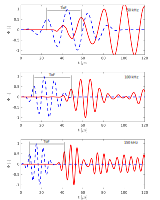
\includegraphics{Chapter_6/ToF_num}
	\end{center}
	\caption{Sensor signals obtained in numerical simulations for the present model.}
	\label{fig:ToF_num}
\end{figure}
\begin{figure}[H]
	\begin{center}
		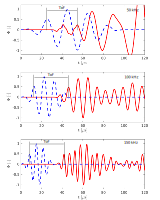
\includegraphics{Chapter_6/ToF_hom}
	\end{center}
	\caption{Sensor signals obtained in numerical simulations for the homogenised model.}
	\label{fig:ToF_hom}
\end{figure}

\begin{table}[H]
	\small
	\tabcolsep=0.25cm
	\centering
	\caption{\label{tab:group_velocity} The group velocities and errors obtain from simulations and experiments.}
	\begin{tabular}{cccccc}
		\toprule
		\textbf{Frequency} & \textbf{Experimental} &\multicolumn{2}{c}{\textbf{Present Model}} & \multicolumn{2}{c}{\textbf{Homogenised Model}}\\
		& C\(_g\) & C\(_g\) & error & C\(_g\) & error\\
		kHz & m/s & m/s & \% & m/s & \%\\
		\midrule
		50  & 5716& 6076& 6.30& 5632& 1.47\\
		100 & 5556& 5985& 7.72& 5938& 6.88\\
		150 & 5402& 5933& 9.83& 5985& 10.79\\
		\bottomrule
	\end{tabular}
\end{table}

\subsection{Efficiency of the time integration algorithm}
Two types of simulations were conducted to determine the efficiency of the \ac{pa} to solve the equation of motion shown in Section \ref{sec:gpu}.
The first type compares the \ac{pa} computations performed on the \ac{gpu} and \ac{cpu}.
The second type compares \ac{pa} with the benchmark proposed by Kudela et al.~\cite{kudela2020parallel} named \ac{ba}.
Both analyses were performed on the same workstation as the \ac{ba} equipped with the following components:
\begin{itemize}
	\item \ac{cpu} - Intel Xeon Silver, 2.1 GHz, 8 cores
	\item \ac{gpu} - NVIDIA Tesla V100 32 GB 5120 CUDA cores
	\item RAM - 128 GB GDDR6
\end{itemize}

The comparison \ac{gpu} vs. \ac{cpu} was conducted on a \ac{3d} model of an  aluminium plate \((250\times250\times 5$ mm$^3)\).
The structure was discretised with rectangular mesh of the various number of the in-plane elements.
In each case, a spectral element of \(6\times 6\times 3\) nodes with three \acp{dof} per node was used, with one element through the plate thickness.
The global \ac{dof} and the memory usage are presented in Table~\ref{tab:gpuvscpu}.
A concentrated force was applied to the centre of the plate as a 3-cycle Hann windowed sine at 50 kHz frequency.
	\begin{table}[!b]
	\tabcolsep=0.25cm
	\centering
	\caption{\label{tab:gpuvscpu} Model parameters used in simulations to compare the algorithm performed on \ac{gpu} and \ac{cpu}.}
	\begin{tabular}{lccccc}
		\toprule
		Elements number & \(25\times25\) & \(50\times50\) & \(100\times100\) &\(125\times125\) &\(250\times250\) \\
		Global \ac{dof}\(\times10^6\) &0.14&0.57&2.26&3.53&14.08\\
		Memory usage [MB] & 75 & 367 & 1437 & 2252 & 8999\\ \bottomrule
	\end{tabular}
\end{table}
The computational speed up as a function of global \ac{dof} was determined as follows:
\begin{eqnarray}
\mathrm{Speedup} = \frac{\mathrm{CPU_{avg}}}{\mathrm{GPU_{avg}}},
\end{eqnarray}
where \(\mathrm{CPU_{avg}}\) and \(\mathrm{GPU_{avg}}\) is average one time step calculation performed on \ac{cpu} and \ac{gpu}, respectively.
The time of the pre-/post-processing is similar for \ac{cpu} and \ac{gpu} because the transfer of data from and to \ac{gpu} is negligible, so it is not included.

For the second test computations run times of the simulations conducted on \ac{gpu} were computed for various sizes of the composite plate.
The benchmark parameters proposed in the paper mentioned above are gathered in Table~\ref{tab:benchmark}.
The efficiency of the \ac{pa} regarding \ac{ba} is measured by speedup, defined as the ratio of \ac{ba} run time to \ac{pa}.
\begin{table}[!t]
\tabcolsep=0.25cm
\centering
\caption{\label{tab:benchmark}Sample parameters used in the benchmark of the \ac{pa} and the \ac{ba}.}
	\begin{tabular}{lcccccc}
		\toprule
		Plate size [cm] & \(30\times30\) & \(40\times40\) & \(50\times50\) & \(70\times70\) & \(90\times90\) & \(100\times100\)\\
		Global \ac{dof}\(\times10^6\)&1.02&1.46&1.98&3.09&5.23&6.36\\ \bottomrule
	\end{tabular}
\end{table}

The results of both analysis are pictured in Fig.~\ref{fig:speedup}.
At maximum \ac{dof}, the speedup in \ac{gpu} computation relative to \ac{cpu} computation increases near to 90 and the \ac{pa} is up to ten more efficient than the \ac{ba}.
Improvement of the algorithm comes from: more operation performed in the preprocessing, transfer of internal forces in the local to the global system by summing columns instead of for-loop, and minimized number of columns in the map of local nodes $\textbf{I}_L$.
\begin{figure}[!tbh]
	\begin{center}
		\includegraphics{Chapter_6/benchmark}
	\end{center}
	\caption{Speedup in function of global \ac{dof} of the \ac{pa} computation in the case of \ac{gpu}~vs.~\ac{cpu} dashed line, and compared to \ac{ba} solid line}
	\label{fig:speedup}
\end{figure}